\chapter{Dynamic Pipeline Framework in Haskell}\label{dp-hs}
One of the fundamental piece of the present work as we have described in ~\autoref{intro} and ~\autoref{prelim},
is the design and implementation of \acrfull{dpfh}: a \acrshort{dpf} written in \acrshort{hs} which allow \acrshort{hs} users
to implement any suitable algorithm in \acrshort{dp}, providing the correct abstractions that helps on that matter.

During the process of conducting this research, we implemented \acrshort{dpfh}~\cite{dynamic-pipeline} and published into 
Hackage (The public Haskell Package Repository of Libraries).
In this chapter we are going to describe the design and implementation details of \acrshort{dpfh}.

\section{Framework Model}

\subsection{Background}
Any suitable library or framework should provide the user the right level of abstraction that removes and hides enough complexity, 
to allow the developer to focus on the problem that it needs to solve.
There are several design approximation to implement a library or framework: \emph{configuration based} where the user only 
focus on follows specific configuration files and provides the runtime system of the framework those configurations to execute the program,
\emph{convention over configuration approach} where the user writes his code and definition following certain pattern in naming or source disposition 
and the framework figures out what needs to be generated on that matter, \emph{functionality based} where the framework or library provides certain amount
of functionality implemented and the user needs to compose those functions to achieve its results and finally \emph{domain specific language models} where 
the framework or library provides a new language that represents the abstraction that we need to deal with. 

In the \emph{domain specific language} approach~\cite{dsl} there exists two types of abstraction: \acrfull{dsl} and \acrfull{edsl}. \acrshort{dsl} or 
usually called external \acrshort{dsl} the propose is to create a completely new language with each own semantic, syntax and interpreter. These are not 
Turing-Complete languages~\cite{turing-comp} because its scope is domain specific as the name indicates. On the other hand \acrshort{edsl} are syntactically 
embedded in the host language of the library, the user writes in the host language library but using the abstractions provided by it with strong checking of 
the constrains imposed by this embedded language.

\acrshort{dpfh} follows a \acrshort{edsl} approach taking advantage of the strong type \acrshort{hs} system giving the user correctness proof at type-level.

\subsection{Framework Design}
In this section we are going to focus on the design of the \acrshort{dpfh} using a \acrshort{edsl} approach. We have built a framework that contains
three important components: \acrshort{dsl}, \acrshort{idl} and \acrshort{rs}. 

\begin{figure}[!ht]
  \centering
  \begin{minipage}{\textwidth}
   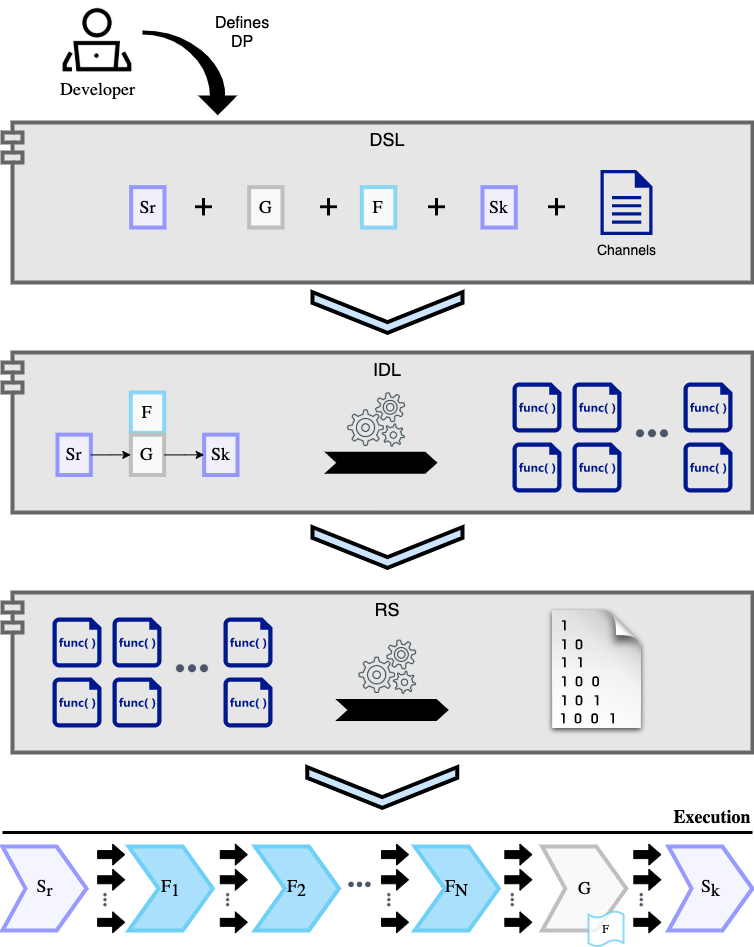
\includegraphics[width=1\textwidth, height=0.6\textheight]{dpf_haskell_v3.png}
    \caption{Architectural view of \acrshort{dpfh}}
    \label{fig:dpfh:1}
  \end{minipage}
\end{figure}

In \autoref{fig:dpfh:1} we can appreciate the different components mentioned before that are the grey boxes.

\paragraph{DSL} The user interacts with the \acrshort{dsl} component where defines how the \acrshort{dp} disposition
should be and what are the channels that are going to communicate the different stages of the pipeline: for example in the
case of \autoref{prole} that we develop the \acrshort{wcc} algorithm, the user knows that is going to received from the Input 
the edges of the graph and it needs two channels between $\iwcc$, $\gwcc$ and $\owcc$, one for sending the edges and another for sending
the accumulated connected components. 

\paragraph{IDL} The user interacts with the \acrshort{idl} which guide him to build the functions with the algorithms needed for each stage: 
$\iwcc$, $\gwcc$, $\owcc$, $\fwcc$ and actors. Based on the definition provided in the \acrshort{dsl}, the framework will indicate the user 
how that definition is interpreted in the context of \acrshort{dp} and what functions should provide.

\paragraph{RS} Once we have the \acrshort{dp} definition and the functions provided by the user with the algorithm solution, the framework
can be fed with this components to execute the program. 

\section{Implementation}
In this section we are going to describe the details of all the techniques used for implementing each of the components described before.
As we have explained in \autoref{sec:contrib}, this library it is published on Hackage~\cite{dynamic-pipeline} and the source code is open 
and can be found on this Github Repository~\cite{dynamic-pipeline-git}.

\subsection{DSL Grammar}\label{sub:sec:dsl-gram}
In order to provide a Type-safe verification in compilation time we have defined a Context Free Grammar that generates a \acrshort{dp} \acrshort{dsl} language  
and it is encoded in custom types. This allows the user to define a type-level \acrshort{dp} of the pipeline he wants to build. 
In order to do that we have the following Context Free Grammar definition.

\begin{definition}[DSL Grammar]
Lets have the grammar $\gdsl = (N, \Sigma, DB, P)$, where $N$ is the set of non-terminal symbols, $\Sigma$ the set of terminal symbols,
$DP \in N$ is the start symbol and $P$ are the generation rules, such that:
\begin{equation*}
    \boxed{
      \begin{aligned}
    N &= \{DP,S_r,S_k,G,F_b,CH,CH_s\},\\
    \Sigma &= \{\text{\mintinline{haskell}{Source}},\text{\mintinline{haskell}{Generator}},\text{\mintinline{haskell}{Sink}},\text{\mintinline{haskell}{FeedbackChannel}},\text{\mintinline{haskell}{Type}},\text{\mintinline{haskell}{Eof}},\text{\mintinline{haskell}{:=>}},\text{\mintinline{haskell}{:<+>}}\},
    \end{aligned}
    }
\end{equation*}
\begin{equation*}
  \boxed{
    \begin{aligned}
  P = \{\\
  DP  &\rightarrow S_r\ \text{\mintinline{haskell}{:=>}}\ G\ \text{\mintinline{haskell}{:=>}}\ S_k\ |\ S_r\ \text{\mintinline{haskell}{:=>}}\ G\ \text{\mintinline{haskell}{:=>}}\ F_b\ \text{\mintinline{haskell}{:=>}}\ S_k,\\
  S_r &\rightarrow \text{\mintinline{haskell}{Source}}\ CH_s,\\
  G   &\rightarrow \text{\mintinline{haskell}{Generator}}\ CH_s,\\
  S_k &\rightarrow \text{\mintinline{haskell}{Sink}},\\
  F_b &\rightarrow \text{\mintinline{haskell}{FeedbackChannel}} CH,\\
  CH_s &\rightarrow \text{\mintinline{haskell}{Channel}}\ CH,\\
  CH &\rightarrow \text{\mintinline{haskell}{Type :<+>}}\ CH\ |\ \text{\mintinline{haskell}{Eof}}\}
\end{aligned}
}
\end{equation*}
\end{definition}

In order to encode this on the language we need to generate encoded it in a Phantom type~\cite{type-index} 
to index the information that we dont want to lose and it is needed for generate the \acrshort{dp}. 
In that sense we create a Phantom type for each element of $\Sigma$.

\begin{listing}[H]
  \begin{minted}[fontsize=\small,numbers=left,breaklines,frame=lines,framerule=2pt,framesep=2mm,baselinestretch=1.2,highlightlines={3,4}]{haskell}

data Source (a :: Type)
data Generator (a :: Type)
data Sink
data Eof
data Channel (a :: Type)
data FeedbackChannel (a :: Type)

  \end{minted}
  \caption{[\mintinline{shell}{Flow.hs}] $\Sigma$ enconding of $G_{dsl}$}
  \label{src:dpfh:1}
\end{listing}
  
As we can see in \autoref{src:dpfh:1}, highlighted types are terminal symbols of $\gdsl$ that are not indexed with any Phantom type. 
This is because they do not carry any extra type information that we need to keep. In the case of \mintinline{haskell}{Sink} it is the last stage
that does not connect further with any other stage, therefore we do not need to indicate channel information. \mintinline{haskell}{Eof} it is just 
a terminal type to disambiguate the \mintinline{haskell}{Channel (a :: Type)} subtree of the full parser tree. Since \mintinline{haskell}{Channel} can carry any type, 
because we need to allow different number of channels and channels types, we need a symbol that marks end of the channel list, i.e. a sum type 
type-level encoded.

There are two more important $\Sigma$ that needs to be addressed independently which are \mintinline{haskell}{:=>} and \mintinline{haskell}{:<+>}.

\begin{listing}[H]
  \begin{minted}[fontsize=\small,numbers=left,breaklines,frame=lines,framerule=2pt,framesep=2mm,baselinestretch=1.2,highlightlines={1,5}]{haskell}

data chann1 :<+> chann2 = chann1 :<+> chann2
  deriving (Typeable, Eq, Show, Functor, Traversable, Foldable, Bounded)
infixr 5 :<+>
   
data a :=> b = a :=> b
  deriving (Typeable, Eq, Show, Functor, Traversable, Foldable, Bounded)
infixr 5 :=>
   
  \end{minted}
  \caption{[\mintinline{shell}{Flow.hs}] $\Sigma$ enconding of $G_{dsl}$ - Especial non-terminals}
  \label{src:dpfh:2}
\end{listing}

In \autoref{src:dpfh:2}, \mintinline{haskell}{:=>} and \mintinline{haskell}{:<+>} can combine 2 types. This types are syntactic sugar and different
because as we are going to see in \acrshort{idl} implementation we need two distinguishable symbols to separate the encoding of the pipeline stage ($\iwcc$, $\gwcc$, $\owcc$)
from the encoding of channel composition in the same stage, as we can appreciate in the $\gdsl$ definition.

As an user and having this few type setup we can start defining our pipelines.  
For example if we want to generate a language for \acrshort{dp} that eliminates duplicated in a stream, we know that
only need one channel connecting the stages that carries the type, in this case \mintinline{haskell}{Int}.

\begin{listing}[H]
  \begin{minted}[fontsize=\small,numbers=left,breaklines,frame=lines,framerule=2pt,framesep=2mm,baselinestretch=1.2,highlightlines={}]{haskell}

type DPExample = Source (Channel (Int :<+> Eof)) 
              :=> Generator (Channel (Int :<+> Eof)) 
              :=> Sink
   
  \end{minted}
  \caption{Example of \acrshort{dp} encoded in $G_{dsl}$}
  \label{src:dpfh:3}
\end{listing}

\subsection{DSL Validation}\label{sub:sec:dsl-val}
The language generated by the grammar needs to be validate in order to avoid the user make mistake and provide an incorrect \acrshort{dp} definition.
Fortunately \acrshort{hs} provides several Type-level techniques~\cite{type-haskell} which allows us to verify properties of our programs in the language before running it, 
saving the users to write bugs and reduce errors. This verification done by the compiler is sophisticated but powerful, establishing a Curry-Howard Isomorphism~\cite{curryhoward}: 
\emph{Propositions as Types - Programs as Proof}. 

Although the language provides a lot of tools to build a type correspondence with propositional logic that can be check at compilation type, it is also known that all these
techniques requires the addition of Language Extensions that serve for that purpose. We cannot forget that even though \acrshort{hs} has more than 20 years of 
Academic Research on its core language, some of the features have been added as extensions, specially the ones that implement state of the art Type Theory concepts. 

The first thing to spot according to the definition on the previous \autoref{sub:sec:dsl-gram} is the validation of the grammar. 
In order to validate the language at type-level we use a \emph{First Class Family}~\cite{associated-types} with a \emph{Type-level Defunctionalization}~\cite{defunctionalization, fun-type-function-haskell} technique.


\begin{listing}[H]
  \begin{minted}[fontsize=\small,numbers=left,breaklines,frame=lines,framerule=2pt,framesep=2mm,baselinestretch=1.2,highlightlines={6,18}]{haskell}

type family And (a :: Bool) (b :: Bool) :: Bool where
    And 'True 'True = 'True
    And a b         = 'False
  

type family IsDP (dpDefinition :: k) :: Bool where
    IsDP (Source (Channel inToGen) :=> Generator (Channel genToOut) :=> Sink)
        = And (IsDP (Source (Channel inToGen))) (IsDP (Generator (Channel genToOut)))
    IsDP ( Source (Channel inToGen) :=> Generator (Channel genToOut) :=> FeedbackChannel toSource :=> Sink)
        = And (IsDP (Source (Channel inToGen))) (IsDP (Generator (Channel genToOut)))
    IsDP (Source (Channel (a :<+> more)))     
        = IsDP (Source (Channel more))
    IsDP (Source (Channel Eof))               = 'True
    IsDP (Generator (Channel (a :<+> more)))  = IsDP (Generator (Channel more))
    IsDP (Generator (Channel a))              = 'True
    IsDP x                                    = 'False
     
type family ValidDP (a :: Bool) :: Constraint where
  ValidDP 'True = ()
  ValidDP 'False = TypeError
                    ( 'Text "Invalid Semantic for Building DP Program"
                      ':$$: 'Text "Language Grammar:"
                      ':$$: 'Text "DP       -> Source CHANS :=> Generator CHANS :=> Sink"
                      ':$$: 'Text "DP       -> Source CHANS :=> Generator CHANS :=> FEEDBACK :=> Sink"
                      ':$$: 'Text "CHANS    -> Channel CH"
                      ':$$: 'Text "FEEDBACK -> FeedbackChannel CH"
                      ':$$: 'Text "CH       -> Type :<+> CH | Eof"
                      ':$$: 'Text "Example: 'Source (Channel (Int :<+> Int)) :=> Generator (Channel (Int :<+> Int)) :=> Sink'"
                    )
  \end{minted}
  \caption{[\mintinline{shell}{Stage.hs}] Validating encoded in $G_{dsl}$ - FCF}
  \label{src:dpfh:4}
\end{listing}

\acrshort{hs} Type system is fully saturated by the compiler, because otherwise it won't type checked in compilation type. 
Before of this our \mintinline{haskell}{IsValid} type as we see in \autoref{src:dpfh:4}, needs to generate the language
of the grammar providing evidence to the Type System that the user must define that language and no other is possible. 
\mintinline{haskell}{IsValid} Type Family saturates to a \mintinline{haskell}{Bool} promoted Type~\cite{promoted-types}, not a boolean value, \mintinline{haskell}{'True} or 
\mintinline{haskell}{'False} with ticks, are promoted types not values. With this technique and defining a custom type level error defined 
in \mintinline{haskell}{ValidDP} type, the compiler will help the user to generate the correct language based on the definition.
Now we can use this types to constraint main functions and ensure the user definition will be type checked by the compiler.

\begin{listing}[H]
  \begin{minted}[fontsize=\small,numbers=left,breaklines,frame=lines,framerule=2pt,framesep=2mm,baselinestretch=1.2,highlightlines={2}]{haskell}

mkDP :: forall dpDefinition filterState filterParam st.
    ( ValidDP (IsDP dpDefinition)
    , DPConstraint dpDefinition filterState st filterParam)
 => Stage (WithSource dpDefinition (DP st)) 
 -> GeneratorStage dpDefinition filterState filterParam st  
 -> Stage (WithSink dpDefinition (DP st))  
 -> DP st ()
mkDP = ...

someFunc = mkDP @DPExample ...

  \end{minted}
  \caption{Using validation of \acrshort{dp} encoded in $G_{dsl}$}
  \label{src:dpfh:5}
\end{listing}

Other details will be cover later in this chapter, but in \autoref{src:dpfh:5} we can appreciate how easy is to constraint over 
the type family defined in the Framework and compiler will show the error if the \acrshort{dp} definition is not correct.

\subsection{IDL}
\acrfull{idl} component takes the definition made on with \acrshort{dsl} grammar to interpret an generate the function definitions, 
that the user needs to fill with their algorithms for solving the specific problem definition. In \autoref{sec:dp} we have describe what are 
the behavior the user needs to provide in a \acrshort{dp} algorithm: each stage ($\iwcc$, $\gwcc$ and $\owcc$) and the $\fwcc$ with the set of Actors, 
that can be 1 or many.

The implementation of \acrshort{idl} helps the user to generate the function definitions that the user needs to complete with the implementation, 
to ensure that those functions will give a Proof of the Propositions defined on the \acrshort{dsl}, therefore the Curry-Howard Correspondence is completed~\cite{curryhoward}.

Similar techniques that we used on \autoref{sub:sec:dsl-val} is also use here. On the first hand we again use type level \emph{Defunctionalization} to 
let the compiler generates the signatures of the required functions and then Term level \emph{Defunctionalization} to interpret that functions.
At the same time some Type Index~\cite{type-index} and Heterogeneous List~\cite{hlist} as also used to keep track of the dynamic number and parameters types of each 
function. 

\begin{listing}[H]
  \begin{minted}[fontsize=\small,numbers=left,breaklines,frame=lines,framerule=2pt,framesep=2mm,baselinestretch=1.2,highlightlines={2,6,10}]{haskell}

withSource :: forall (dpDefinition :: Type) st. WithSource dpDefinition (DP st) 
            -> Stage (WithSource dpDefinition (DP st))
withSource = mkStage' @(WithSource dpDefinition (DP st))

withGenerator :: forall (dpDefinition :: Type) (filter :: Type) st. WithGenerator dpDefinition filter (DP st) 
              -> Stage (WithGenerator dpDefinition filter (DP st))
withGenerator = mkStage' @(WithGenerator dpDefinition filter (DP st))

withSink :: forall (dpDefinition :: Type) st. WithSink dpDefinition (DP st) 
           -> Stage (WithSink dpDefinition (DP st))
withSink = mkStage' @(WithSink dpDefinition (DP st))
  \end{minted}
  \caption{[\mintinline{shell}{Stage.hs}] Using withXXXX Interpreters of \acrshort{dp} encoded in $G_{dsl}$}
  \label{src:dpfh:6}
\end{listing}

As we can see on \autoref{src:dpfh:6} there is \mintinline{haskell}{Stage *} class type that we use for 
the Defunctionalization at term level, and that class is polymorphic in the type of Stage it can build.
The differents \mintinline{haskell}{WithSource}, \mintinline{haskell}{WithGenerator} and \mintinline{haskell}{WithSink}
\emph{Associated Type Families}~\cite{associated-types} help the compiler to deduce the signature of the function that the user should provide for that Stage.


\begin{listing}[H]
  \begin{minted}[fontsize=\small,numbers=left,breaklines,frame=lines,framerule=2pt,framesep=2mm,baselinestretch=1.2,highlightlines={7,11}]{haskell}

type family WithSource (dpDefinition :: Type) (monadicAction :: Type -> Type) :: Type where
  WithSource (Source (Channel inToGen) :=> Generator (Channel genToOut) :=> Sink) monadicAction
      = WithSource (ChanIn inToGen) monadicAction
  WithSource (Source (Channel inToGen) :=> Generator (Channel genToOut) :=> FeedbackChannel toSource :=> Sink) monadicAction 
      = WithSource (ChanOutIn toSource inToGen) monadicAction
  WithSource (ChanIn (dpDefinition :<+> more)) monadicAction         
      = WriteChannel dpDefinition -> WithSource (ChanIn more) monadicAction
  WithSource (ChanIn Eof) monadicAction                              
      = monadicAction ()
  WithSource (ChanOutIn (dpDefinition :<+> more) ins) monadicAction  
      = ReadChannel dpDefinition -> WithSource (ChanOutIn more ins) monadicAction
  WithSource (ChanOutIn Eof ins) monadicAction                       
      = WithSource (ChanIn ins) monadicAction
  WithSource dpDefinition _                                          
      = TypeError
          ( 'Text "Invalid Semantic for Source Stage"
            ':$$: 'Text "in the DP Definition '"
            ':<>: 'ShowType dpDefinition
            ':<>: 'Text "'"
            ':$$: 'Text "Language Grammar:"
            ':$$: 'Text "DP       -> Source CHANS :=> Generator CHANS :=> Sink"
            ':$$: 'Text "DP       -> Source CHANS :=> Generator CHANS :=> FEEDBACK :=> Sink"
            ':$$: 'Text "CHANS    -> Channel CH"
            ':$$: 'Text "FEEDBACK -> FeedbackChannel CH"
            ':$$: 'Text "CH       -> Type :<+> CH | Eof"
            ':$$: 'Text "Example: 'Source (Channel (Int :<+> Int)) :=> Generator (Channel (Int :<+> Int)) :=> Sink'"
          )
  \end{minted}
  \caption{[\mintinline{shell}{Stage.hs}] WithSource Associate Type Details}
  \label{src:dpfh:7}
\end{listing}

In \autoref{src:dpfh:7} we can see in the highlighted lines how the type induction is 
expanding a function definition of the form \mintinline{haskell}{a -> b -> ...} depending on 
\acrshort{dp} language definition. Lets see how \mintinline{haskell}{Stage} was defined in order 
to read saturate this type and ask the user the proper function according to that generated type.

\begin{listing}[H]
  \begin{minted}[fontsize=\small,numbers=left,breaklines,frame=lines,framerule=2pt,framesep=2mm,baselinestretch=1.2,highlightlines={12,16}]{haskell}

data Stage a where
  Stage :: Proxy a -> a -> Stage a

mkStage' :: forall a. a -> Stage a
mkStage' = Stage (Proxy @a)
    
  \end{minted}
  \caption{[\mintinline{shell}{Stage.hs}] Stage Data Type}
  \label{src:dpfh:8}
\end{listing}

It is use a simple \mintinline{haskell}{Proxy a} phantom type technique to remember the type definition generated by \mintinline{haskell}{a}.
In the case of \mintinline{haskell}{withSource} interpreter shown in \autoref{src:dpfh:6}, $\mintinline{haskell}{a} \thicksim \mintinline{haskell}{WithSource definition}$, therefore 
when compiler fully saturates the type it can tell the user what is the function that \mintinline{haskell}{Stage} should contain.

\paragraph{Generator and Filter}
Generator ($\gwcc$) and Filter ($\fwcc$) should be explain together because as we have seen on \acrshort{dp} definition in \autoref{sec:dp},
$\gwcc$ has a $\fwcc$ template in order to know how to dynamically interpose a new $\fwcc$ during the runtime execution of the program.
Lets first study $\fwcc$ Data Type in the context of the framework.

\begin{listing}[H]
  \begin{minted}[fontsize=\small,numbers=left,breaklines,frame=lines,framerule=2pt,framesep=2mm,baselinestretch=1.2,highlightlines={2,5}]{haskell}

newtype Actor dpDefinition filterState filterParam monadicAction =
    Actor {  unActor :: MonadState filterState monadicAction => Stage (WithFilter dpDefinition filterParam monadicAction) }

newtype Filter dpDefinition filterState filterParam st =
    Filter { unFilter :: NonEmpty (Actor dpDefinition filterState filterParam (StateT filterState (DP st))) }
    deriving Generic
    
  \end{minted}
  \caption{[\mintinline{shell}{Stage.hs}] Filter / Actor Data Type}
  \label{src:dpfh:9}
\end{listing}
$\fwcc$ is a list \mintinline{haskell}{NonEmpty} list of \mintinline{haskell}{Actor}. This is exactly represented as the \acrshort{dp} theoretical definition.
Some things that needs to be highlighted from this \autoref{src:dpfh:9}. On the first hand \mintinline{haskell}{Actor} is an \mintinline{haskell}{Stage} which is 
also obvious since it is the Actor the stage that is going to interpose between the $\gwcc$ and the previous Filters. Moreover \mintinline{haskell}{Stage} on \mintinline{haskell}{Actor}
is going to be defunctionalized with \mintinline{haskell}{WithFilter} \emph{Associated type family} with the same concept as we have seen before for the other stages. In this
sense the user of the framework will be able to type check the actor functions (proof) that needs to provide to the framework according to the language definition.
On the other hand, \mintinline{haskell}{Filter} has explicit \mintinline{haskell}{StateT} monadic context. This is because the $\fwcc$ instance could store something in its local state 
during the execution, for example in the case of $\dpwcc$ as we seen in \autoref{prole} $\fwcc$ keeps an updated list of connected components that updates as long as it receives more edges.
Some combinators and smart constructors are provided in the framework to facilitate the construction of $\fwcc$ and Actors as we can see in \autoref{src:dpfh:10}

\begin{listing}[H]
  \begin{minted}[fontsize=\small,numbers=left,breaklines,frame=lines,framerule=2pt,framesep=2mm,baselinestretch=1.2,highlightlines={}]{haskell}

mkFilter :: forall dpDefinition filterState filterParam st. WithFilter dpDefinition filterParam (StateT filterState (DP st)) 
         -> Filter dpDefinition filterState filterParam st
mkFilter = Filter . single

single :: forall dpDefinition filterState filterParam st. WithFilter dpDefinition filterParam (StateT filterState (DP st)) 
       -> NonEmpty (Actor dpDefinition filterState filterParam (StateT filterState (DP st)))
single = one . actor

actor :: forall dpDefinition filterState filterParam st. WithFilter dpDefinition filterParam (StateT filterState (DP st)) 
      -> Actor dpDefinition filterState filterParam (StateT filterState (DP st))
actor = Actor . mkStage' @(WithFilter dpDefinition filterParam (StateT filterState (DP st)))

(|>>>) :: forall dpDefinition filterState filterParam st. Actor dpDefinition filterState filterParam (StateT filterState (DP st)) 
       -> Filter dpDefinition filterState filterParam st 
       -> Filter dpDefinition filterState filterParam st
(|>>>) a f = f & _Wrapped' %~ (a <|)
infixr 5 |>>>

(|>>) :: forall dpDefinition filterState filterParam st. Actor dpDefinition filterState filterParam (StateT filterState (DP st)) 
      -> Actor dpDefinition filterState filterParam (StateT filterState (DP st)) 
      -> Filter dpDefinition filterState filterParam st
(|>>) a1 a2 = Filter (a1 <|one a2)
infixr 5 |>>
  \end{minted}
  \caption{[\mintinline{shell}{Stage.hs}] Filter / Actor smart constructors and combinators}
  \label{src:dpfh:10}
\end{listing}

Now $\gwcc$ contains a $\fwcc$ template that we have explained before and its own stage behavior.

\begin{listing}[H]
  \begin{minted}[fontsize=\small,numbers=left,breaklines,frame=lines,framerule=2pt,framesep=2mm,baselinestretch=1.2,highlightlines={}]{haskell}
data GeneratorStage dpDefinition filterState filterParam st = GeneratorStage
    { _gsGenerator      :: Stage (WithGenerator dpDefinition (Filter dpDefinition filterState filterParam st) (DP st))
    , _gsFilterTemplate :: Filter dpDefinition filterState filterParam st
    }  
  \end{minted}
  \caption{[\mintinline{shell}{Stage.hs}] Generator}
  \label{src:dpfh:11}
\end{listing}

\subsection{RS - Runtime System}
The \acrshort{rs} can be divided in two parts: the combinators that allows in runtime generate dynamically stages as long as data arrives to $\gwcc$
and the execution context of the \acrshort{dp}.

Regarding execution context, all the stage that we have seen in previous sections are the pieces needed to build an executable \mintinline{haskell}{DP st a} monad.
This executable monad has an existential type similar to \mintinline{haskell}{ST} monad to not scape out from the context on different stages.

Once the dynamic pipeline start to execute the core of the framework is to dynamically generate stage according to the user definition between $\gwcc$ and previous 
stages (at the beginning only the $\iwcc$ is before $\gwcc$). This is not more than an \emph{anamorphism}~\cite{lenses} that creates $\fwcc$ instance until some condition is met.

\begin{listing}[H]
  \begin{minted}[fontsize=\small,numbers=left,breaklines,frame=lines,framerule=2pt,framesep=2mm,baselinestretch=1.2,highlightlines={2,12,14,15,16,17,18}]{haskell}
unfoldF :: forall dpDefinition readElem st filterState filterParam l. SpawnFilterConstraint dpDefinition readElem st filterState filterParam l
        => UnFoldFilter dpDefinition readElem st filterState filterParam l 
        -> DP st (HList l) 
unfoldF = loopSpawn

where
  loopSpawn uf@UnFoldFilter{..} =
    maybe (pure _ufRsChannels) (loopSpawn <=< doOnElem uf) =<< DP (pull _ufReadChannel)

  doOnElem uf@UnFoldFilter{..} elem' = do
    _ufOnElem elem'
    if _ufSpawnIf elem'
     then do
       (reads', writes' :: HList l3) <- getFilterChannels <$> DP (makeChansF @(ChansFilter dpDefinition))
       let hlist = elem' .*. _ufReadChannel .*. (_ufRsChannels `hAppendList` writes')
       void $ runFilter _ufFilter (_ufInitState elem') hlist (_ufReadChannel .*. (_ufRsChannels `hAppendList` writes'))
       return $ uf { _ufReadChannel = hHead reads', _ufRsChannels = hTail reads' }
     else return uf

  \end{minted}
  \caption{[\mintinline{shell}{Stage.hs}] unfoldF}
  \label{src:dpfh:12}
\end{listing}

In \autoref{src:dpfh:12} we can see that the \mintinline{haskell}{unfoldF} receives an \mintinline{haskell}{UnFoldFilter}
Data type, which contains the recipe for controlling that unfold recursive call. In line 12, we can see that one of that 
elements of the recipe is when to stop recursion. Inside the conditional in the first line we create new channels for that filter,
because as \acrshort{dp} states we need to create new channels for connect this new filter computation with the previous and with the next, 
therefore the next stage are going to be fed with the new channels of this filter. After that we run the filter to put the computation 
to work in the pipeline and finally we return the new channels to the next stage, which is going to be $\gwcc$.
As we can also be appreciated in the code there is an intensive use of \mintinline{haskell}{HList}~\cite{hlist}. This is because since the \acrshort{dp}
definition made by the user dynamically generates the functions of the different stages, we have indexed its type and number of parameters
using Heterogeneous Lists and in particular the library \mintinline{shell}{HList}.
The same as $\fwcc$ and Actors, we have created combinators to generate different \mintinline{haskell}{UnFoldFilter} recipes. 

\begin{listing}[H]
  \begin{minted}[fontsize=\small,numbers=left,breaklines,frame=lines,framerule=2pt,framesep=2mm,baselinestretch=1.2,highlightlines={}]{haskell}
mkUnfoldFilter :: (readElem -> Bool) 
    -> (readElem -> DP st ()) 
    -> Filter dpDefinition filterState filterParam st 
    -> (readElem -> filterState)
    -> ReadChannel readElem
    -> HList l 
    -> UnFoldFilter dpDefinition readElem st filterState filterParam l


mkUnfoldFilterForAll' :: (readElem -> DP st ())
                      -> Filter dpDefinition filterState filterParam st
                      -> (readElem -> filterState)
                      -> ReadChannel readElem
                      -> HList l
                      -> UnFoldFilter dpDefinition readElem st filterState filterParam l

mkUnfoldFilterForAll :: Filter dpDefinition filterState filterParam st
                      -> (readElem -> filterState)
                      -> ReadChannel readElem
                      -> HList l
                      -> UnFoldFilter dpDefinition readElem st filterState filterParam l
   \end{minted}
  \caption{[\mintinline{shell}{Stage.hs}] UnfoldFilter combinators}
  \label{src:dpfh:13}
\end{listing}

In \autoref{src:dpfh:13} the first combinator is the default smart constructor. First parameter \mintinline{haskell}{(readElem -> Bool)} indicate if the a new filter should 
be spawn or not. Second parameter \mintinline{haskell}{(readElem -> DP st ())} is a monadic optional computation to do when received an element, for example loging.
Next to that is the Filter. \mintinline{haskell}{(readElem -> filterState)} is given the first element that the filter will be spawn, what is the initial state of the filter.
Each filter is feed mainly by a \mintinline{haskell}{(ReadChannel readElem)} from where to receive elements, and finally the Heterogeneous list with the rest of the channels to 
connect with other stages.
\mintinline{haskell}{mkUnfoldFilterForAll} is to indicate to the framework that for each element received in the Generator a new filter should be spawn. 

\section{Libraries and Tools}
\subsection{Parallelization} 
One of the most important components of the implementation is the selection of a concurrency library to support an intensive parallelization workload. Parallelization techniques and tools have been intensively studied and implemented in \acrshort{hs} \cite{monadpar}. Indeed, it is well known that green or light threads and spark allow for spawning thousands to millions of parallel computations. These parallel computations do not penalize performance when compare with \acrfull{os} level threading \cite{parallelbook}. 
A straightforward assumption to achieve this could be to use \texttt{monad-par} library \cite{monadparlib, monadpar}. Nevertheless, in this experimental work, we have discarded the use of sparks \cite{sparks} because we can achieve the level of required parallelism spawning green threads only. This is caused by the nature of \acrshort{dp}, where pipeline parallelism and not data parallelism is a structural processing mechanism. The next obvious choice is to use \mintinline{haskell}{forkIO :: IO () -> IO ThreadId} from \texttt{base} library \cite{forkio}. However, that would imply handling all the threads lifecycle, terminations, and errors programmatically without major combinators or abstractions to deal with them. Therefore, we choose \texttt{async} library \cite{async}  which enables to spawn asynchronous computations \cite{parallelbook} on \acrshort{hs} and at the same time, it provides useful combinators to managing thread terminations and errors.

\subsection{Channels\label{section:channels}} 
We have several techniques to our disposal to communicate between threads or sparks in \acrshort{hs} like \mintinline{haskell}{MVar} or concurrent safe mechanisms like \acrfull{stm} \cite{stm}. Moreover, we have at our disposal \textit{Channels} abstractions based on both mentioned communication techniques. In that sense, for conducting the communication between dynamic stages and data flowing in a $\DP$, we have selected \texttt{unagi-chan} library \cite{unagi} which provides the following advantages to our solution: Firstly,  \mintinline{haskell}{MVar} channel without using \acrshort{stm}. This allows avoiding internal locking for concurrent access. In this case, we can use this advantage because in a $\DP$, one specific stage which is running in a separated thread, can only access to its \textit{I/O} channels for reading/writing accordingly and those operations are not concurrently shared by other threads (stages) for the same channels. Second,  non-blocking channels. \texttt{unagi-chan} library contains blocking and non-blocking channels for reading. This aspect is key to gain speed up on the implementation. Third, the library is optimized for $x86$ architectures with use of low-level \texttt{fetch-and-add} instructions. Finally, \texttt{unagi-chan} is $100x$ faster on Benchmarking compare with \acrshort{stm} and default base \mintinline{haskell}{Chan} implementations.

\section{Chapter Summary}
In this chapter we have describe with great level of detailed how \acrlong{dpfh} has been conceived from a Design point of view, 
as well as all the \acrshort{hs} data types and language techniques that we use for that implementation. At the end of the chapter we mentioned external libraries used for the runtime system.
